\documentclass[12pt]{article}
\usepackage[utf8]{inputenc}
\usepackage{float}
\usepackage{amsmath}
\usepackage{amssymb}
\usepackage{tikz}

\usepackage[hmargin=3cm,vmargin=6.0cm]{geometry}
%\topmargin=0cm
\topmargin=-2cm
\addtolength{\textheight}{6.5cm}
\addtolength{\textwidth}{2.0cm}
%\setlength{\leftmargin}{-5cm}
\setlength{\oddsidemargin}{0.0cm}
\setlength{\evensidemargin}{0.0cm}

%misc libraries goes here
\usepackage{fitch}

\begin{document}

\section*{Student Information } 
%Write your full name and id number between the colon and newline
%Put one empty space character after colon and before newline
Full Name :  Alperen OVAK\\
Id Number :  2580801\\

% Write your answers below the section tags
\section*{Answer 1}

The \( Q_n \) cube graph has \( 2^n \) vertices, and each vertex is labelled with a binary string of lenght n, each vertices is connected to other vertices whose labels is differ in exactly one digit.

To derive a recurrence relation for the number of edges \( E_n \) in \( Q_n \), consider how we can form \( Q_n \) from \( Q_{n-1} \).

The cube graph \( Q_n \) can be constructed by taking two copies of \( Q_{n-1} \) and connecting corresponding vertices in these two copies by an edge.

Considering:

\begin{enumerate}
    \item \( Q_{n-1} \) has \( 2^{n-1} \) vertices and \( E_{n-1} \) edges.
    \item When adding another dimension to \( Q_{n-1} \), we essentially have two identical \( Q_{n-1} \) graphs.
    \item We need to relabel those vertices. Let add a leading 0 for one of the \( Q_{n-1} \) and 1 for other \( Q_{n-1} \)
    \item Since before adding leading number we had pairs whose labels are same but not connected, after adding leading number those pairs differ in exactly one digit. Therefore we need to connect them. \\
    \[
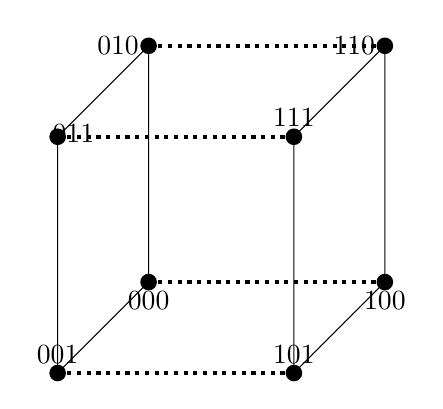
\begin{tikzpicture}[scale=1.5]
    % Define vertices and labels
    \coordinate[label=below:000] (000) at (0,0,0);
    \coordinate[label=above:001] (002) at (0,0,2);
    \coordinate[label=left:010] (020) at (0,2,0);
    \coordinate[label={[shift={(0.2,-0.2)}]above:011}] (022) at (0,2,2);
    \coordinate[label=below:100] (200) at (2,0,0);
    \coordinate[label=above:101] (202) at (2,0,2);
    \coordinate[label=left:110] (220) at (2,2,0);
    \coordinate[label=above:111] (222) at (2,2,2);

   \foreach \point in {(000),(002),(020),(022),(200),(202),(220),(222)} {
        \fill \point circle[radius=2pt];
    }
    % Draw edges
    \draw (000) -- (002) -- (022) -- (020) -- cycle;
    \draw (200) -- (202) -- (222) -- (220) -- cycle;
    \draw[dotted, line width=1.5pt]  (000) -- (200);
    \draw[dotted, line width=1.5pt] (002) -- (202);
    \draw[dotted, line width=1.5pt] (020) -- (220);
    \draw[dotted, line width=1.5pt] (022) -- (222);
\end{tikzpicture}
\]
    \item To connect corresponding vertices in these two \( Q_{n-1} \) graphs to form \( Q_n \), we need to add \( 2^{n-1} \) edges.
\end{enumerate}

Therefore, the total number of edges \( E_n \) in \( Q_n \) is:
\[ E_n = E_{n-1} + 2^{n-1} \]

This represents the recurrence relation for the number of edges in the \( Q_n \) cube graph in terms of \( E_{n-1} \). \\ \\


\section*{Answer 2}

To find the generating function for the sequence
\[ <1, 4, 7, 10, 13, \ldots >\]
We can use the formula for an arithmetic sequence.

The \( n^{th} \) term of an arithmetic sequence can be represented as:
\[ a_n = a_1 + (n - 1) \cdot d \]
where:
\begin{align*}
a_n & \text{ is the } n^{th} \text{ term of the sequence}, \\
a_1 & \text{ is the first term of the sequence}, \\
n & \text{ is the term number (position)}, \\
d & \text{ is the common difference between consecutive terms}.
\end{align*}
From the given sequence, we can observe that:
\[ a_1 = 1 \] (first term)
and
\[ d = 3 \] (since the difference between consecutive terms is 3).

Plugging these values into the formula, we get:
\[ a_n = 1 + (n - 1) \cdot 3 \]
which simplifies to:
\[ a_n = 1 + 3n - 3 \]
and further simplifies to:
\[ a_n = 3n - 2 \]

Starting with the basic generating functions:
\begin{enumerate}
    \item The generating function for the sequence \( <1, 1, 1, 1, \dots> \) is:
    \[ \frac{1}{1-x} \]

    \item Differentiating the above generating function gives:
    \[ \frac{d}{dx} \left( \frac{1}{1-x} \right) = \frac{1}{(1-x)^2} \]
    Which represents the sequence \( <1, 2, 3, 4, \dots> \).

    \item Using the scaling theorem:
    \begin{align*}
    &\text{Multiplying } \frac{1}{1-x} \text{ by 2 gives:} \\
    &\frac{2}{1-x} \\
    &\text{Which represents the sequence } <2, 2, 2, 2, \dots>.
    \end{align*}

    \begin{align*}
    &\text{Multiplying } \frac{1}{(1-x)^2} \text{ by 3 gives:} \\
    &\frac{3}{(1-x)^2} \\
    &\text{Which represents the sequence } <3, 6, 9, 12, \dots>.
    \end{align*}

    \item Subtracting the generating function for the sequence \( <2, 2, 2, 2, \dots> \) from the generating function for the sequence \( <3, 6, 9, 12, \dots> \) gives:
    \[ \frac{3}{(1-x)^2} - \frac{2}{1-x} \]
    This resulting generating function represents the sequence \( <1, 4, 7, 10, 13, \dots> \).
\end{enumerate}

Therefore, \( \frac{1+2x}{(1-x)^2} \)  is the generating function for the sequence \( <1, 4, 7, 10, 13, \dots> \).



\section*{Answer 3}

Define the generating function for the sequence \( a_n \) as:
\[ A(x) = \sum_{n=0}^{\infty} a_n x^n \]

Multiply both sides of the recurrence relation by \( x^n \) and sum over all valid values of \( n \):
\begin{align*}
\sum_{n=1}^{\infty} a_n x^n &= \sum_{n=1}^{\infty} a_{n-1} x^n + \sum_{n=1}^{\infty} 2^n x^n \\
\end{align*}

\begin{align*}
&= x\sum_{n=1}^{\infty} a_{n-1} x^{n-1} + \sum_{n=1}^{\infty} 2^n x^n
\end{align*}

We can write \( \sum_{n=1}^{\infty} a_{n-1} x^{n-1}\) as \( \sum_{n=0}^{\infty} a_{n} x^{n} = A(x) \) \\

Furthermore, we know that  \( \sum_{n=0}^{\infty} 2^n x^n = \frac{1}{1-2x} \),\\

Thus \( \sum_{n=1}^{\infty} 2^n x^n = \frac{1}{1-2x} - 1\)\\

Let's put them into the equation we have above:

\begin{align*}
A(x)-a_{0} &= xA(x) + \frac{1}{1-2x} - 1\\
A(x)-1 &= xA(x) + \frac{1}{1-2x} - 1\\
A(x)(1-x) &= \frac{1}{1-2x}\\
\end{align*}

Therefore, \( A(x) \) is:

\begin{align*}
A(x)&= \frac{1}{(1-2x)(1-x)} = \frac{B}{(1-x)} + \frac{C}{(1-2x)}  \ \ B,C \in \mathbb{R}\\
\end{align*}

So, we have \( B=-1\) and \(C=2\)

\begin{align*}
A(x)&= \frac{1}{(1-2x)(1-x)} = \frac{-1}{(1-x)} + \frac{2}{(1-2x)}  \\
\end{align*}

Since sequence of \( \frac{1}{1-x} \) generating function is \( <1, 1, 1, 1, \dots> \),\\

Sequence of \(\frac{-1}{(1-x)}\) is \( <-1, -1, -1, -1, \dots> \).\\

Since sequence of \( \frac{1}{1-2x} \) generating function is \( <1, 2, 4, 8, \dots> \),\\

Sequence of \(\frac{2}{(1-2x)}\) is \( <2, 4, 8, 16, \dots> \).\\

Therefore sequence of \( A(x) \) is \[ <1, 3, 7, 15, \dots, 2^{n+1}-1 , \dots>\].\\
Thus, we can say that: \[ a_n = 2^{n+1}-1\]



\section*{Answer 4}

\section*{Answer 5}


\end{document}
